%! Author = adam
%! Date = 28.02.21

\chapter{Channeling}\label{ch:channeling}

Last chapter we discussed the stochastic process of a ion beam as it collides with atoms within a crystal/sample.
But what happens if the incident beam of ions is perfectly aligned in the 'gaps' of a crystalline lattice?
The german word for this phenomena I think fits quite well: Gitterfuehrungseffekt, i.e., to pass through the lattice.
A diagram of when this is to happen is found in Figure~\ref{fig:channel1}.
Basically, the ion is constrained on its path through a crystalline solid.
This is not the case for amorphous solids (non crystalline) as there we would have the effects described in the previous chapter.
\begin{figure}
	\begin{subfigure}{0.5\textwidth}
		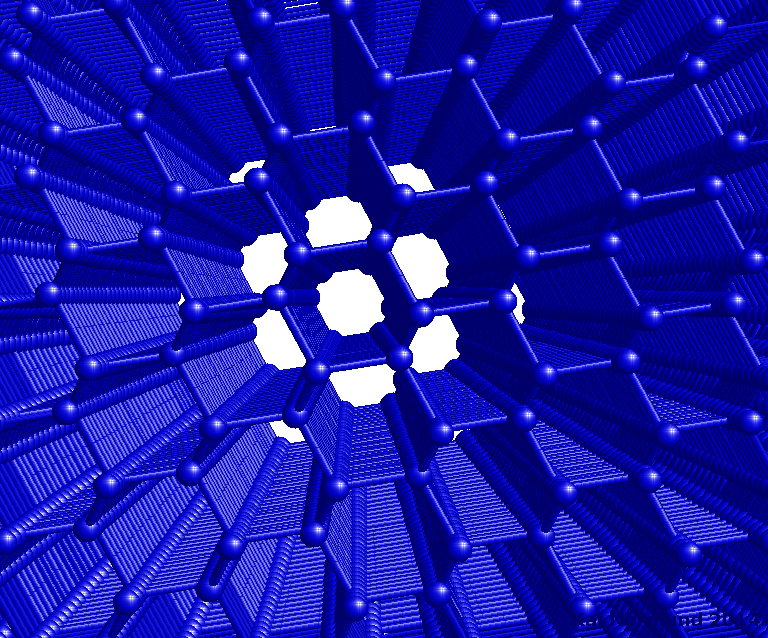
\includegraphics[width=0.9\linewidth, height=5cm]{SC1}
		\caption{An about 12 nm thick silicon crystal viewed down the 110 crystal direction.}
		\label{fig:SC1}
	\end{subfigure}
	\begin{subfigure}{0.5\textwidth}
		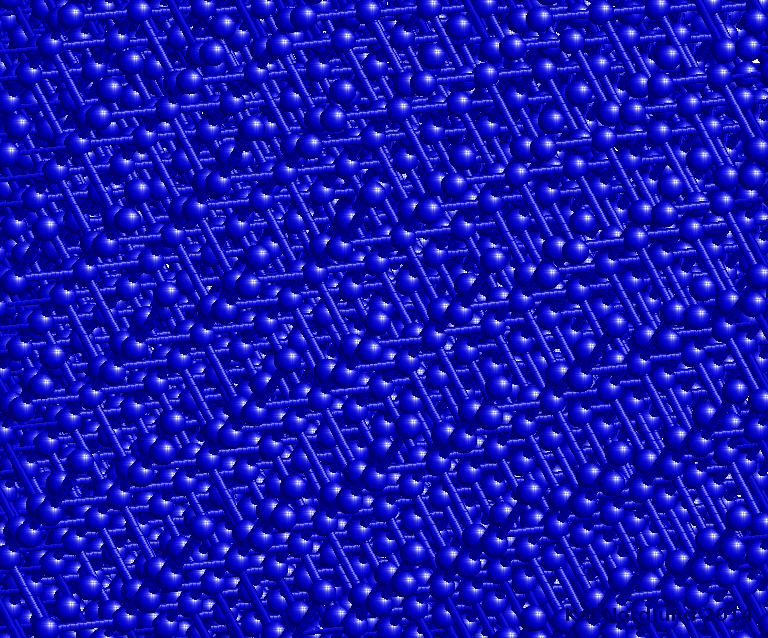
\includegraphics[width=0.9\linewidth, height=5cm]{SC2}
		\caption{The same Si crystal, but viewed from a randomly rotated direction}
		\label{fig:SC2}
	\end{subfigure}
	\caption{POV of an ion coming to hit a crystal from two different angles. Taken from wikipedia}
	\label{fig:channel1}
\end{figure}
 The influence of the crystal lattice not only appears in the orientation of the lattice, but also in the vibrational amplitude of the lattice atoms (T).
Additionally, properties like surface preparation, beam divergence, and disorder introduced by the implantation itself can lead to changes in the channeling effect.

In channeling, we have a much lower energy loss, i.e, stopping power.
This leads to a greater range in which the particle can travel through the sample.
Due to this, we have less resulting nuclear stopping, and thus less damage to the sample.
\section{Continuum Model}\label{sec:continuum-model}
Also called axial channeling, the continuum model
The trajectory of a channeled particle is described mathematically below but schematically in Figure~\ref{fig:trajec}

\begin{figure}
	\centering
	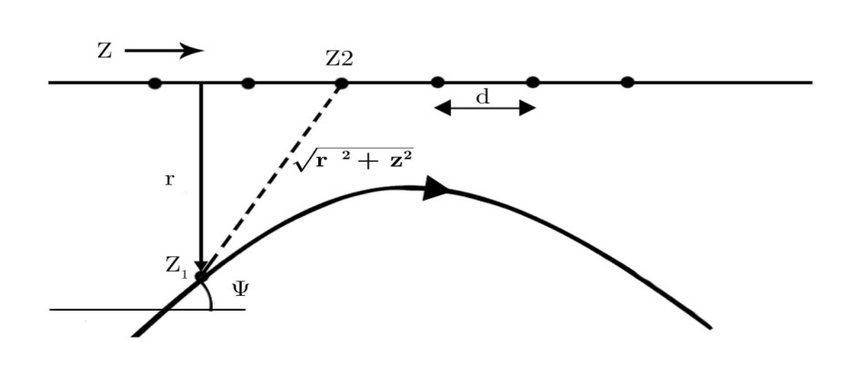
\includegraphics{trajectory}
	\caption{Trajectory of a channeled particle}
	\label{fig:trajec}
\end{figure}
As they travel through the 'channel', ions feel a screened potential, $U$,  given by:
$$U(r) = \frac{Z_1 Z_2 e^2}{4\pi\epsilon_0 d} \ln \left[ \left( \frac{\sqrt{3}a}{r}\right)^2 + 1\right]$$
where $d$ is the spacing between atoms within their planes, $a$ is the Thomas-Fermi radius.
We can use conservation of energy to determine the critical angle $\Psi_c$ between the plane between two planes in which the ion will oscillate around.
$$ E = \frac{p_{\parallel} ^2}{2m} + \frac{p_{\perp} ^2}{2m}  + U(r)$$
where $p_\parallel = p\cos\Psi$, $p_\perp = p\sin\Psi$.
This yields us:
$$ E = \frac{p^2 \cos^2 \Psi}{2m} + \frac{p^2 \sin^2 \Psi}{2m} + U(r)  \underbrace{\rightarrow}_{\Psi << 1} \frac{p^2 \Psi^2}{2m} +  \frac{p^2 \Psi^2}{2m} + U(r) \underbrace{\rightarrow}_{\textrm{perp. part}}  E_\perp \approx \frac{p^2\Psi^2}{2m} + U(r) $$
Th minimum distance $r_m$ where the channeling breaks down (i.e., where $\Psi_c$ is), is then:
$$ \frac{p^2\Psi_c^2}{2m} = E\Psi_c^2  \overset{!}{=} U(r_m) \Rightarrow \Psi_c = \sqrt{\frac{U(R_m)}{E}}$$
How do we find $r_m$? If $r_m$ is approximately in the range of the thermal vibrational amplitudes of lattice atoms then the channeling breaks down.
Therefore if we assume \textunderscore{isotropic} thermal amplitudes, then the mean square vibrational amplitude $\langle u^2 \rangle$ will yield us:
$$r_m \approx \rho = \sqrt{\langle x^2 \rangle + \langle y^2 \rangle} - \sqrt{ \frac{2}{3} \langle u^2 \rangle} $$
and finally:
$$\Psi_c = \sqrt{\frac{2Z_1 Z_2 e^2}{4\pi \epsilon_0 d E}} \sqrt{\frac{1}{2} \ln \left( \frac{\sqrt{3} a}{\rho}\right) + 1}$$
Since $a$ is normally on the order of 0.01 mm, and $\rho$ on the order 0.005 mm, then the right square root is approximately 1.

The continuum model can be broken down into three broad categories.
Group \textbf{A}: There is strong interaction with the lattice, and the range distribution is similar to that of an amorphous material.
Group \textbf{B}: the ion starts with large oscillations in the channel, followed by a high probability to be de-channeled at some point.
Group \textbf{C}: these ions are 'well' channeled, i.e., there is a good chance to remain channeled during the whole slowdown process.
How does an ion beam join one of these three groups?
Well for that we have a little table:

\begin{table}[h]
	\centering
	\begin{tabular}{c | c | c }
		\hline
		Group & Angle & Position \\
		\hline
		A & $\Phi_A > \Phi_C$ & close to atomic rows \\
		B & $\Phi_B < \Phi_{cr}$ & slightly further away to atomic rows \\
		C & $\Phi_C < \Phi_B < \Phi_{cr}$ & near the channel center
	\end{tabular}
	\caption{The angle is that relative to the midline between the two crystal lattice planes.  }
    \label{tab:Continuum}
\end{table}
Dechanneled, which just means that the ion, either abruptly or at the end of its range, leaves its channeled path.
This can occur at any point during the channeled ions' life, i.e., there is a probability for it to just de-channel, and in some cases it is more likely to do so than other (see group B of continuum model).
There are some maximum ranges that come with channeling, if we have a 50--150 keV ion beam and good alignment to the main crystal axis, then the range of the ion depth is 2--50 times greater than that of an amorphous solid!
Also, the stopping of channeled ions (de-channeling) is determined by electronic stopping.
If we recall from previous chapters, near the end of the ions' life in the sample, this is where electronic stopping occurs.
This leads us to the stopping power relations of:
$$\underbrace{S_e}_\textrm{channeled} << \underbrace{S_e + S_n}_\textrm{amorphous} $$
where $S_e$ and $S_n$ are the electronic and nuclear stopping powers respectively.

One can also use de-channeling to investigate defects of samples.
Imagine the rows of atoms are not so neat, and we were to have some defects, i.e., atoms are not aligned on the plane.
If we were to have one of these defects, then the channeling that was to be assumed to be fine, there would in fact be maybe a backscattering event, or the ion becomes de-channeled and is no longer in the crystal channel.
One can measure the proportion of the beam that is channeled vs not channeled (scattered for example), we can learn something about the crystal quality, and the defects relative to the crystal.
This can be seen in Figure~\ref{fig:dech}

\begin{figure}
	\centering
	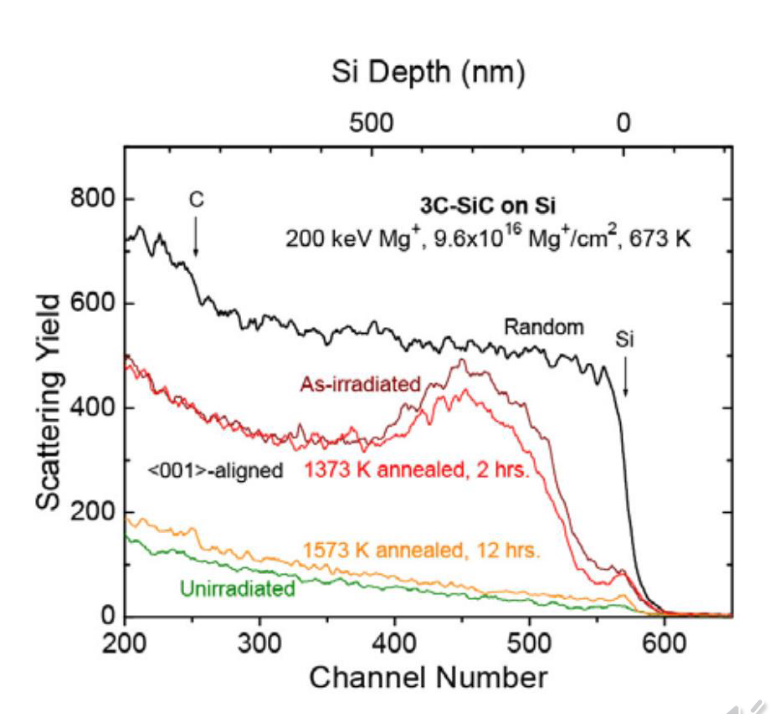
\includegraphics[scale=0.35]{dechannel}
	\caption{Here we have a silicon sample with various types of defects implemented in the sample that is being fired upon with a 200 keV helium beam ion. On the y-axis we have the backscattered ions, and the x-axis the number of channeled ions. The black line (random) is with random orientation of the ion beam so we have high number of back scattered atoms. For an non irradiated sample without any disorder, we have a low number of backscattered ions. Annealing is discussed later chapters but we note here that over a time, the annealing repairs the damage from the implantation (red lines) such that we are back to having a high amount of channeled atoms compared to those backscattered.}
	\label{fig:dech}
\end{figure}

\section{Example: Diamond}\label{sec:example:-diamond}
In Leipzig there is a lot of work done using diamond, which has two crystal planes that work well for channeling: $\langle 100 \rangle$ and $\langle 111 \rangle $.
After plugging in numbers from literature, we can find our $\Psi_c \approx 6^{\deg} $ for E$\approx 200$keV of an Argon ion beam in Diamond.
\section{Summary}\label{sec:summary6}
\begin{wrapfigure}{r}{0.5\textwidth}
	\centering
	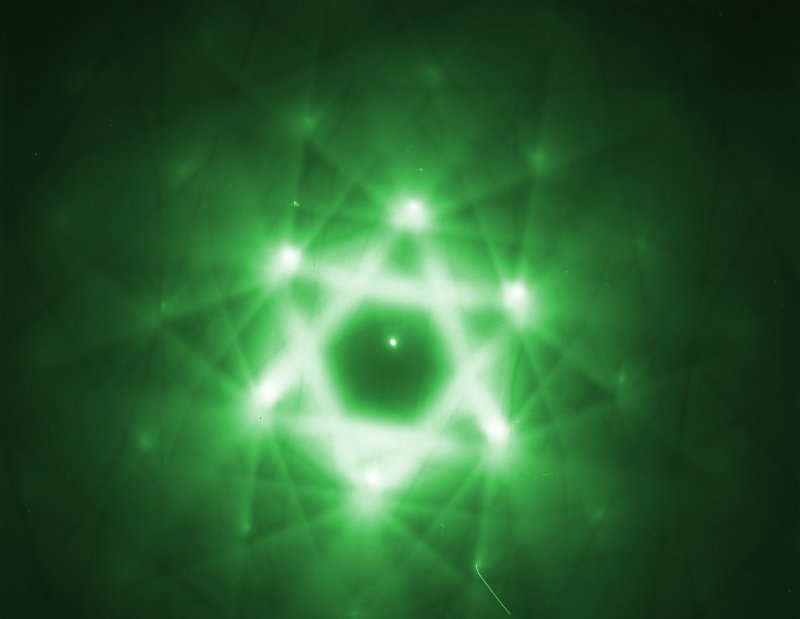
\includegraphics[scale=1.3]{BZ_ion}
	\caption{The brillouin zone construction by 300keV electrons. }
\end{wrapfigure}
Fun fact this was discovered initially through computer simulations.
There are several interesting application of channeling.
Channeling effects can be used as tools to investigate porerties of the crystal lattice and of its perturbations (like doping) not accessible to X-rays.
It may also be utilized to detect geometrical abnormalities in crystals, and is a variation of Rutherford Backscattering.
Channeling can even super-focus ion beams for sub-atomic microscopy.
At higher energies (tens of GeV), the applications include channeling radiation for enhanced production of high energy gamma rays, and the use of bent crystals for extraction of particles from particle accelerators.

\begin{myitemize}
	\item If ions hit at just the right angle to a crystal lattice, then they will be channeled, i.e., will follow a relatively linear path without being scattered and displacing other atoms
	\item There are three main groups of ions impact that result in scattering, based off of angle and the position relative to crystal plane
	\item Channeling is due to the Coulomb potential felt by the ion as it travels between the plane, leading it to an oscillatory motion.
\end{myitemize}
